
\chapter{Conclusion --- orthography}
\label{cha:orth-concl}

Part~\ref{part:orthography} demonstrated that the orthography of lenition may be employed to establish the date of composition of \gls{mw} texts. These developments are summarised in Table~\ref{tab:arolwg}. Any \gls{mw} text consistently applying any of the patterns described in this table may be dated to its appropriate period.

\begin{table}[h]
  \centering
  \begin{tabular}{rcccl}
    \toprule
    \multicolumn{1}{c}{Period} & \tch{\xT} & \tch{\lT} &  \tch{\xD} & \multicolumn{1}{c}{Other \gls{l}\gls{C}} \\
    \midrule
    \gls{ow} & \mw{p, t, c} & \mw{{p, t, c}} & \mw{b, d, g} & {Not represented} \\
    <1275\hphantom{--1325}  & \mw{p, t, c} & \mw{{p, t, c}} & \mw{b, d, g} & Represented, except /d, r̥/ \\
    1275--1325  & \mw{p, t, c} & \mw{{p, t,} {g}} & \mw{b, d, g} & Represented, except /d, r̥/ \\
    >1325 & \mw{p, t, c} & \mw{{b, d, g}} & \mw{b, d, g} & Represented, except /d, r̥/\\
    \gls{mow} & \mow[]{p, t, c}& \mow[]{b, d, g} &\mow[]{b, d, g} & Represented\\
    \bottomrule
  \end{tabular}%
  \caption{The orthographical development of lenition.}
  \label{tab:arolwg}
\end{table}

This account depends on \gls{mw} texts consistently employing a single orthography of lenition. Such straightforwardness is only found when the date of its original composition is in the same period as its extant manuscript witness. The corpus of Chapter~\ref{cha:indep-comp-mwbr} had these features and so it gave an impression of the orthographical standard of different stages in the \gls{mw} period. In most \gls{mw} texts, however, such a short gap between the original composition of a text and its extant manuscript witnesses is uncommon.

Most \gls{mw} manuscripts postdate the twelfth century, even if the texts they contain are much older. In such cases instances of lenition may be represented due to modernising tendencies of later scribes. Chapter~\ref{cha:welsh-laws} showed  that such modernisations are incomplete, \ie the pattern of lenition of the original composition is still visible. Different scribes would modernise the orthography of lenition to different extents, but the extent of modernisation never reached 100\%\footnote{See \eg Figure~\ref{fig:barchartlaws} on page~\pageref{fig:barchartlaws}.}. This makes even a minority of unlenited \mw[]{p, t, c} instead of \mw[]{b, d, g} indicative of composition before the thirteenth century. A singular instance of orthographic lenition has lower evidential value than a singular instance of lack thereof, because a scribe may have been quite thorough in modernising.

Some manuscript texts are copies of copies, so they may show the traces of more than one stage of modernisation. A possible example of this is law manuscript \gls{sK}, a fifteenth-century manuscript with partial lenition of all voiceless stops. Based on this alone, we may conclude that its original composition predates the mid-thirteenth century, yet representation of lenition of \mw[]{c} is comparatively more widespread than \mw[]{p, t}. This may be evidence that an intermediate copy written in the late thirteenth century existed as a base for manuscript \gls{sK}.

Scribes modernising the orthography of lenition did so inconsistently. The same word may be found lenited and unlenited in the same manuscript, even when both words should be lenited according to our knowledge of \gls{mw}. Similarly, an element known to cause lenition may have orthographical lenition following it inconsistently. Chapter~\ref{cha:stemm-mwbuch-dewi} demonstrated that this randomly added orthographical lenition may be employed to reconstruct the stemmatics of multiple manuscript witnesses of a single text.

Whenever a scribe added lenition randomly, he would create a unique fingerprint of instances of lenition that were and were not orthographically represented. Thus, if we find a sufficiently similar pattern of lenition and non-lenition in a manuscript, they may share a common intermediate ancestor in which such a fingerprint was formed. The existence of such a shared fingerprint may be differentiated from chance correspondences with statistical tests, but a shared fingerprint may also have its roots in a convergent development of otherwise unrelated manuscripts.

\section{Dating the orthographical shift and the phonological shift}
\label{sec:change-lenition-as}

Part~\ref{part:orthography} treated the orthographical change of lenited \mw[]{p, t, c} from \mw[]{p, t, c} to \mw[]{b, d, g}. Although the insights of Part~\ref{part:phonology-phonetics} make it obvious that this change in orthography reflected a change in phonology at some point, it is not necessarily the case that the changes occurred at the same time. Orthography typically lags behind orthography, and the case of Modern English orthography shows that several hundred years of phonological development may be obscured by orthography.

Still, there is some evidence that the change in orthography did not lag behind the change in phonology much. The treatment of lenited \mw[]{g} and how lenition was sometimes consciously not written so that a reader would not misread and have to repair his reading\footnote{See Section~\ref{sec:lenited-mwg}}. The case of lenited \mw[]{g} demonstrates that thirteenth-century scribes did not write lenition by choice, rather than simply because they had not invented the means yet. In the face of this, it is not a stretch to assume that writing \lT\ with \mw[]{p, t, c} served a similar purpose in ensuring correct pronunciation as \lT; not \xD. This gives reason to believe that the orthographical shift of \lT\ from \mw[]{p, t, c} to \mw[]{b, d, g} lagged very little --- if at all --- behind the phonological shift of \lT\ to \xD.

Another reason to assume the orthographical development had a concurrent development in phonology is that the shift in orthography is somewhat reminiscent of how phonological innovations spread through lexical diffusion. Table~\ref{tab:lexdiffxw} gives an example of how the sound change /χʷ > w/ in mid Wales occurred at different stages at successive points in time at a single location. The columns may also be thought of as representing different geographical locations along the path of change~\todo{pagenumber}\autocite{Wil_Lexical05}. The merger of \lT\ with \xD\ can be represented using a similar table, which is illustrated by Table~\ref{tab:stagesltxd}.


\begin{table}[h]
  %% https://tex.stackexchange.com/questions/433930/stepped-table-in-booktabs/
  \centering
  \begin{tabular}{wwwwq}
    \toprule
    \tch{\(t_1\)} & \tch{\(t_2\)} & \tch{\(t_3\)} & \tch{\(t_4\)} & \tch{gloss} \\
    \midrule
     χware & \multicolumn{1}{|w}{ware} & ware & ware & play\\\cline{2-2}
     χwanen & χwanen & \multicolumn{1}{|w}{wanen} & wanen & flea\\\cline{3-3}
    χwa:ir & χwa:ir & χwa:ir & \multicolumn{1}{|w}{wa:ir} &sister\\
    \bottomrule
  \end{tabular}%
  \caption{Lexical diffusion of /χʷ > w/, adapted from \textcite{Wil_Lexical05}, based on \textcite[214--16]{Che_time77}. \(t_1, t_2\) et cetera represent successive points in time at a single location.}
  \label{tab:lexdiffxw}%
\end{table}%


\begin{table}[h]
  \centering
  \begin{tabular}{wwwwq}
    \toprule
    \tch{\(t_1\)} & \tch{\(t_2\)} & \tch{\(t_3\)} & \tch{\(t_4\)} & \tch{gloss} \\
    \midrule
    can, i cyd & \multicolumn{1}{|w}{gan, i gyd} & gan, i gyd & gan, i gyd & with, together\\\cline{2-2}
    ei coron & ei coron & \multicolumn{1}{|w}{ei goron} & ei goron & his crown \\\cline{3-3}
    ei plu & ei plu & ei plu & \multicolumn{1}{|w}{ei blu}& his feathers \\
    ei tad & ei tad & ei tad & \multicolumn{1}{|w}{ei dad}& his father \\
    \bottomrule
  \end{tabular}%
  \caption{Discernible intermediate stages of the merger between \lT\ and \xD\ in \gls{mw}.}
  \label{tab:stagesltxd}
\end{table}

The orthographical shift of  \lT\  to \xD\ is comparable to lexical diffusion in that it initially applied to a limited set of words or phonemes, and then gradually grew to cover more environments. Lexical diffusion of sound change is a phenomenon observed to exist in spoken language, so if the \gls{mw} written language shows this phenomenon, then it is probable that it also existed in the spoken language of its day.

\begin{table}[h]
  \centering
  \begin{tabular}{IIIIIIIq}
    \toprule
    \tch{\(t_1\)} & \tch{\(t_2\)} & \tch{\(t_3\)} & \tch{\(t_4\)} & \tch{\(t_5\)} & \tch{\(t_6\)} & \tch{\(t_7\)} & \tch{gloss} \\
    \midrule
    ik & \multicolumn{1}{|I}{ich} & ich & ich & ich & ich & ich & I \\\cline{2-2}
    maken & maken & \multicolumn{1}{|I}{machen} & machen & machen & machen & machen & make \\\cline{3-3}
    dorp & dorp & dorp & \multicolumn{1}{|I}{dorf} & dorf & dorf & dorf & village \\\cline{4-4}
    dat & dat & dat & dat & \multicolumn{1}{|I}{das} & das & das & that \\\cline{5-5}
    appel & appel & appel & appel & appel & \multicolumn{1}{|I}{apfel} & apfel & apple \\\cline{6-6}
    pund & pund & pund & pund & pund & pund & \multicolumn{1}{|I}{pfund} & pound \\
    \bottomrule
  \end{tabular}%
  \caption{Discernible intermediate dialect areas in the High German Consonant Shift.}
  \label{tab:hgcstable}%
\end{table}%


Another development comparable to the merger between \gls{mw} \lT\ and \xD\  is the dialectology of the \gls{hgcs}. The \gls{hgcs} involved the Proto-Germanic voiceless stops /p t k/\footnote{It also involved  voiced spirants /β ð ɣ/, but I restrict myself to the voiceless stops here.} . In word-initial position, medially following a consonant, or when doubled, the voiceless stops developed into their corresponding affricates: High German /pf, ts, kx/. Medially between vowels and word-finally, voiceless stops became voiced fricatives: /f, s, x/~\autocite[56--57]{Wat_History76}.  This shift may obviously be called a single shift, in that we may describe it as a general shift from stops towards their corresponding affricates and fricatives (among others). Yet isoglosses separating High German from Low German (the latter of which did not undergo the \gls{hgcs}) show that intermediate dialects underwent some, but not all of these developments. the impact of the \gls{hgcs} increases gradually to the South, and different consonants are affected to different degrees. Figure~\ref{fig:hgcsmap} and Table~\ref{tab:hgcstable} give an impression of some intermediate dialects. Not all developments are included, however. The extent of \eg~/k > kx/ is even more limited to the Southern area~\autocite[56n]{Wat_History76}.

\begin{figure}[h]
  \centering
  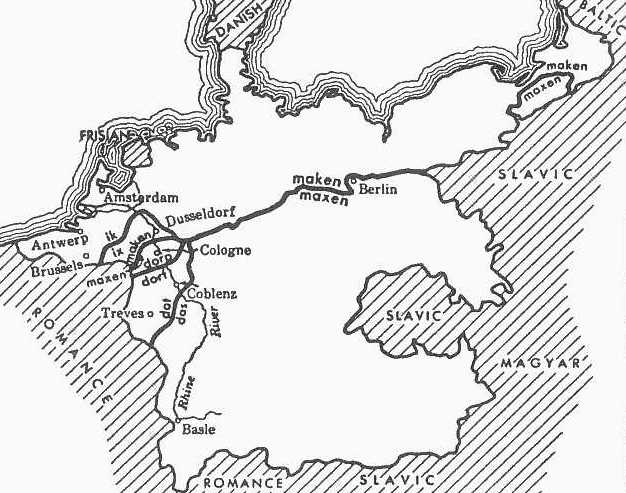
\includegraphics[width=0.8\textwidth]{3orth/images/hgcs.jpg}
  \caption[Bloomfield's isoglosses of the \gls{hgcs}.]{The Dutch-German speech area, with the isoglosses of several words containing [k/x], [t/s], and [p/f], from \textcite[344]{Blo_Language33}}
\label{fig:hgcsmap}
\end{figure}

\section{Geography and chronology of the shift}
\label{sec:geogr-chron-shift}

In the \gls{hgcs} we see a single shift of consonants, realised at different levels of completeness in different geographical locations. The merger of \lT\ and \xD\ in \gls{mw} has a temporal rather than a geographical transition zone. Yet the \gls{hgcs} did not occur overnight either:
\tqt{The spread of the High German shift northward, whatever its ultimate provenience, took place slowly. Although we have demonstrated the occurrence of shifted forms in Alemannic territory for as early as 600, we must not supose that this change was thoroughgoing and complete at this time. [\dots] Bavarian documents preserve some non-High German forms well into the eighth century and even later. [\dots] And not until the ninth century did the High German consonant shift reach the Middle Franconian dialect.}{Wat_History76}{62}
The fact that the \gls{hgcs} is executed to different levels of completeness along both temporal and geographical axes raises the question what the initial geographical extent of the merger of \lT\ to \xD\ was in \gls{mw}. This matter has remained unsolved in Part~\ref{part:orthography}, but it is obvious that some geographically intermediate stages must have existed for some amount of time.


\section{A review of \gls{mw} lenition rules}
\label{sec:cons-other-ideas}
Knowledge of when orthographical lenition of voiceless stops was introduced in Welsh, and knowledge of how scribes would emend older texts after this introduction makes it necessary to reconsider what we think we know of \gls{ow} and \gls{mw} grammar. I give an example below.

\Textcite[2]{schrijver_free_2010}, citing \textcite[18, 179]{evans_grammar_1964} and \textcite[193n]{morgan_y_1952}, states:
`Normally, if a plural subject noun follows the verb, the verb is in the 3sg [\dots]. In early poetry, a plural verb may precede a plural subject, in which case the subject undergoes lenition.' Evidence for this archaic rule comes from the sentences below:
\begin{mwl}
  \mwc[ex:schrsubplv1]{CLlH 23.5a}{yn Aber Cuawc yt ganant gogeu}{In Aber Cuawg cuckoos sing}
  \mwc[ex:schrsubplv2]{AP 5.141}{ymgetwynt Gymry}{the Welsh will see to it}
\end{mwl}

The Canu Llywarch Hen poems are thought to have been composed in \gls{ow}, even though they survive in \gls{mw} orthography and in fourteenth century manuscripts, and the Book of Taliesin is shown to have added orthographic lenition of \mw[]{c}\todo{I must refer to this if I describe it elsewhere}. Having established that  lenition of voiceless stops was represented in the thirteenth century at the earliest, and having established that fourteenth-century scribes would add orthographical lenition of voiceless stops, we must amend Schrijver's (and Evans' and Morgan's) statement that nominal subjects of plural verbs undergo lenition in early poetry.

The fact of the matter is that lenition was probably added by the fourteenth-century manuscript scribes, rather than the original composers of the poem. It is indeed a feature of early poetry that plural verbs may have nominal subjects, but the lenition following it is not a feature of the early poetry itself, but rather a feature of the fourteenth-century manuscripts.

This means that those seeking to prove early poetry indeed had lenition of nominal subjects following plural verbs would either need to find a lenited nominal subject that has an initial consonant other than \mw[]{p, t, c}, or they would need to demonstrate that the orthographic lenition of these consonants indeed precedes the fourteenth century. In fact, \textcite[65--66]{van_development14} does not find subject lenition following plural verbs, but finds instances of non-lenition instead, including one case other than \mw[]{p, t, c}:
\mwcc[ex:vansluissubjlen]{RBH 641.38}{A gwrhau a \al{orugant gwyr} y iarllaeth y owein.}{And the noblemen did fealty to Owain’s earldom.}
This example comes from the Red Book of Hergest, dating from around 1400, and the tale itself is much younger than the examples given by Schrijver. This curious mix of lenition and non-lenition remains an elusive puzzle, but all the pieces in this puzzle discovered so far belong to the \gls{mw} period, not the \gls{ow} period. Solving this puzzle would improve our knowledge of fourteenth-century Welsh, but it would not directly shed light upon the grammar of \gls{ow}\footnote{The examples quoted here curiously show lenition of voiceless stops, and non-lenition of other consonants. If this is indeed the pattern found, then subject lenition following plural verbs may not be representative of any synchronic stage of Welsh, but may instead be how fourteenth-century scribes thought the older stage operated. Then, when updating the orthography of lenition, they would use contemporary orthography for lenition, but non-contemporary rules governing lenition.}.

\section{Further research}
\label{sec:further-research}
\begin{itemize}
\item The problem of creating categories of lenition, see Buchedd Dewi
\item What is the geographical source of the merger between \lT\ and \xD? Were there any transition areas in the thirteenth century?
\item What other preconceptions about rules governing lenition need to be reviewed in the light of later scribes adding lenition to earlier texts?
\end{itemize}
% \section{Salesbury}
% \label{sec:salesbury}

% Fisher says:
% \tqt{Prefaced to the Prayer Book of 1567 is given his promised `Explanation of certaine wordes being quareled withall', from which we take the following:

%   `Vy-Dew for vynnuw, or vynyw, wherein D is now reteined, euen for the more significatiue expressing of the grace of the woord.

%   Vy-popul for vymhobl, to saue the word the les maimed.
  
%   Vy-troet for vynrhoed that the signification may be more apparent to the straunge Reader'.

%   It is clear that he wanted the reader --- the silent reader particularly --- to see what the original form of the word was, not only as regards the initial letter, but also in compounds, as we find. This method, he, of course, applied to the written word only, that it might be self-explanatory, and he never meant that any one should read aloud the text actually as written. Rather, he expected the reader to be himself able to introduce the proper mutations as i the spoken language, which any intelligent Welshman could and would do, and so read correctly without the imputed \textit{llediaith} and \textit{anghyfiaith}. By thus writing the words so as to indicate their supposed etymology, he also though that Welsh people of both North and South Wales would be the better able to understand them. In fact, he concerned himself with written Welsh only, and wanted to preserve the words `the les maimed' and `uncorrupt', without the mutations, regardless of the fact that the language as a living organism must grow and change with time, and in accordance with its own genius.
% }{Fis_Kynniver31}{xxxvii--xxxviii}

% \tqt{He treats compounds and words that are not compounds in the same manner. After all he was simply following the earlier orthography; \eg [\dots] \textit{ympren croc, yn tuy vyntat, vygkorffi, amperffaith}.}{Fis_Kynniver31}{xxxix}

% Professor Richards' review:
% \tqt{In 1567, evidently in answer to his critics, he demanded, ``who \dots\ dyd ever wryte euery words as he sounded it?''. Another innovation was equally infelicitous. A stranger learning Welsh finds that the consonantal changes at the beginning of a word constitute his chief difficulty. Thus the word for father is written \textit{tad, dad, thad,} or \textit{nhad} according to its position in a sentence. Salesbury in every case used the radical or simplest form of such words. To judge from a sentence in the Dedication prexied to his Dictionary his object was to render it easier for readers to look up unusual words. The result was disastrous . His language appear clumsy and ungrammatical and the Welsh people would have none of it. Partly for this reason, and partly because it was superseded by Biship Richard Davies's translation of the whole Prayer Book in 1567, Kynnifer Llith a Ban was but little used.}{Ric_Welsh31}{}



%%% Local Variables:
%%% coding: utf-8
%%% mode: latex
%%% TeX-master: "../main"
%%% End:
